\documentclass[12pt,]{article}
\usepackage{lmodern}
\usepackage{amssymb,amsmath}
\usepackage{ifxetex,ifluatex}
\usepackage{fixltx2e} % provides \textsubscript
\ifnum 0\ifxetex 1\fi\ifluatex 1\fi=0 % if pdftex
  \usepackage[T1]{fontenc}
  \usepackage[utf8]{inputenc}
\else % if luatex or xelatex
  \ifxetex
    \usepackage{mathspec}
  \else
    \usepackage{fontspec}
  \fi
  \defaultfontfeatures{Ligatures=TeX,Scale=MatchLowercase}
\fi
% use upquote if available, for straight quotes in verbatim environments
\IfFileExists{upquote.sty}{\usepackage{upquote}}{}
% use microtype if available
\IfFileExists{microtype.sty}{%
\usepackage{microtype}
\UseMicrotypeSet[protrusion]{basicmath} % disable protrusion for tt fonts
}{}
\usepackage[margin=0.50in]{geometry}
\usepackage{hyperref}
\hypersetup{unicode=true,
            pdftitle={Analysis of integration site distributions and clonal abundances for gene therapy correction of cystinosis},
            pdfauthor={John K. Everett, Ph.D.~and Frederic Bushman, Ph.D.},
            pdfborder={0 0 0},
            breaklinks=true}
\urlstyle{same}  % don't use monospace font for urls
\usepackage{graphicx,grffile}
\makeatletter
\def\maxwidth{\ifdim\Gin@nat@width>\linewidth\linewidth\else\Gin@nat@width\fi}
\def\maxheight{\ifdim\Gin@nat@height>\textheight\textheight\else\Gin@nat@height\fi}
\makeatother
% Scale images if necessary, so that they will not overflow the page
% margins by default, and it is still possible to overwrite the defaults
% using explicit options in \includegraphics[width, height, ...]{}
\setkeys{Gin}{width=\maxwidth,height=\maxheight,keepaspectratio}
\IfFileExists{parskip.sty}{%
\usepackage{parskip}
}{% else
\setlength{\parindent}{0pt}
\setlength{\parskip}{6pt plus 2pt minus 1pt}
}
\setlength{\emergencystretch}{3em}  % prevent overfull lines
\providecommand{\tightlist}{%
  \setlength{\itemsep}{0pt}\setlength{\parskip}{0pt}}
\setcounter{secnumdepth}{0}

%%% Use protect on footnotes to avoid problems with footnotes in titles
\let\rmarkdownfootnote\footnote%
\def\footnote{\protect\rmarkdownfootnote}

%%% Change title format to be more compact
\usepackage{titling}

% Create subtitle command for use in maketitle
\newcommand{\subtitle}[1]{
  \posttitle{
    \begin{center}\large#1\end{center}
    }
}

\setlength{\droptitle}{-2em}

  \title{Analysis of integration site distributions and clonal abundances for
gene therapy correction of cystinosis}
    \pretitle{\vspace{\droptitle}\centering\huge}
  \posttitle{\par}
    \author{John K. Everett, Ph.D.~and Frederic Bushman, Ph.D.}
    \preauthor{\centering\large\emph}
  \postauthor{\par}
      \predate{\centering\large\emph}
  \postdate{\par}
    \date{October 2018}

\usepackage{booktabs}
\usepackage{longtable}
\usepackage{array}
\usepackage{multirow}
\usepackage[table]{xcolor}
\usepackage{wrapfig}
\usepackage{float}
\usepackage{colortbl}
\usepackage{pdflscape}
\usepackage{tabu}
\usepackage{threeparttable}
\usepackage{threeparttablex}
\usepackage[normalem]{ulem}
\usepackage{makecell}

\usepackage{caption}

\begin{document}
\maketitle

{
\setcounter{tocdepth}{2}
\tableofcontents
}
\captionsetup[table]{labelformat=empty}

\newpage

\section{Summary of results}\label{summary-of-results}

The goal of this analysis is to investigate the integration profile of a
gene therapy vector for the correction of cystinosis in mouse subjects
and assess potential clonal expansions. The list of mouse oncogenes was
compiled from the retroviral tagged cancer gene database
(RTCGD)\textsuperscript{1} using an inclusion threshold of three or more
incidents where the mouse oncogene list comprises 2.01\% of all mouse
genes. The frequency of integration near oncogenes was generally less
than that of mice in a previously published \(\beta\)-thalassemia mouse
trial from which no adverse events have been reported
\textsuperscript{2}. The code base for this analysis is available online
(\href{https://github.com/everettJK/project.geneTherapy.ucsdMouseCystinosis}{link}).

\vspace{0.25cm}

Twenty-nine mice were tested by serial transfer of vector-treated bone
marrow. From these, 64,413 cells were sampled, yielding 3,647 total
unique integration sites. In both donor and recipient samples, there was
no overall increase in integration sites near annotated murine
cancer-associated genes, thus providing no evidence for genotoxicity.
Some cells expanded more than others, but analysis of cells showing the
most pronounced expansion showed no enrichment in integration sites in
or near cancer-associated genes. In one case, decendants of a single
cell appears to have mainly repopulated a test mouse (pCN801). This cell
appears to have harbored \textasciitilde{}12 independent integration
events, and proliferated robustly, so that the final specimen showed a
VCN of 9.58. Upon transfer to a recipient mouse (pCN951), the cell clone
proliferate sluggishly (VCN 0.083), suggesting that despite the number
of integration events, no major change in growth properties took place.
None of the 12 genes are annotated as cancer associated genes. Specimens
of integration into human cells in culture were also compared (VIS UCSD
CYS Report.group1). Results showed no favored integration near cancer
associated genes compared to previous studies of integration site
distributions. Thus the tests of integration site distributions here
provide no strong evidence for genotoxicity of the vector analyzed
greater than for vectors used safely to date in ongoing human trials.

\newpage

\section{Mouse samples studied}\label{mouse-samples-studied}

Integration sites were detected in 29 samples from mouse subjects
(Tables 1 \& S1).

\vspace{0.1cm}

\begin{table}[!h]

\caption{\label{tab:unnamed-chunk-2}Table 1. Overview of data collection.}
\centering
\begin{tabular}[t]{ccccc}
\toprule
Organism & Number of samples & Number of reads & Number of inferred cells & Number of integration sites\\
\midrule
mouse & 29 & 16,317,429 & 64,413 & 3,647\\
\bottomrule
\end{tabular}
\end{table}

\vspace{0.5cm}

\section{Subject reports}\label{subject-reports}

Subject specific reports for all subjects are available via a protected
web archive
(\href{http://www.bushmanlab.org/data/export/cherqui}{link}).\\
user: cherqui\\
pass: geneTherapy@!\#

\vspace{0.5cm}

\section{UCSC browser exploration}\label{ucsc-browser-exploration}

UCSC browser sessions pre-loaded with the integration sites identified
in this analysis are available via this\\
(\href{http://genome.ucsc.edu/cgi-bin/hgTracks?org=mouse\&db=mm9\&hgt.customText=http://microb120.med.upenn.edu/UCSC/cherqui/UCSC_CYS_mouse.group2.ucsc}{link}).
Integration sites are shown as blue (positive orientation integration)
and red (reverse orientation integration) tick marks. For each
integration site, a second track provides the maximum clonal abundance.
Entering gene names into the search bar will direct the browser to
specific genes.

\newpage

\section{Description of analysis
techniques}\label{description-of-analysis-techniques}

We investigate effects of integration on cell growth using the following
criteria: Integration Frequency is the frequency at which unique
integration sites are observed in or near a given gene. Clonal Abundance
is determined by quantifying the number of sites of linker ligation
associated with each unique integration site. This samples the number of
DNA chains at the start of the experiment allowing clonal expansion to
be quantified\textsuperscript{4}.

Relative clonal Abundance is determined per sample and is the percentage
of identified cells attributed to a given clone. Integration sites and
the clones harboring them are sampled from a larger population. It would
be rare for all integration sites in a sample to be represented in the
sequence data.

For this analysis, four technical replicates of each delivered sample
were prepared, sequenced and analyzed with the INSPIIRED integration
site analysis pipeline (v1.2)\textsuperscript{4}.

\newpage

\section{Comparisons to previous
trials}\label{comparisons-to-previous-trials}

\subsection{Integration events near oncogenes in mouse
subjects}\label{integration-events-near-oncogenes-in-mouse-subjects}

\vspace{0.1cm}

In order to determine if the experimental vector has a higher propensity
of integrating near suspected oncogene in mice than previously employed
vectors, the frequency of integration near oncogenes was compared to a
previously published mouse trial\textsuperscript{2} which used a
comparable lentiviral vector to correct \(\beta\)-thalassemia. The
frequency of integration events near oncogenes in the subjects was less
than the mean frequency of integration events near oncogenes in the
published trial (Figure 1 {[}experimental subjects: gray, previous
\(\beta\)-thalassemia trial: blue{]}).

\vspace{1.0cm}

\emph{Figure 1. Comparison of frequencies of integration events near
oncogenes.}

\vspace{0.5cm}

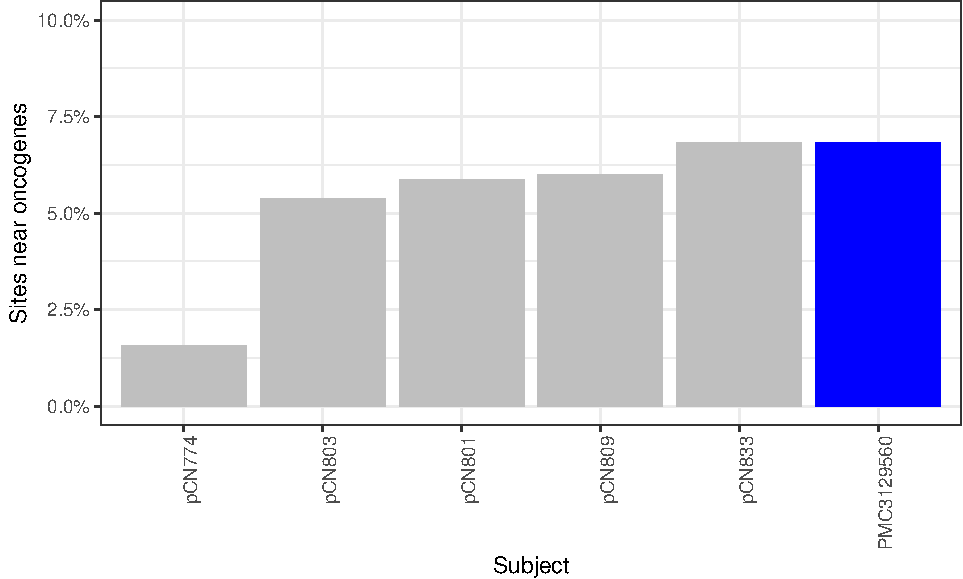
\includegraphics{project.group2_files/figure-latex/fig1-1.pdf}

\newpage

\section{Relative abundances of mouse subject
samples}\label{relative-abundances-of-mouse-subject-samples}

The sample relative abundance plots below (Figure 2) show the most
abundant 25 clones in each sample as colored bars while less abundant
clones were relegated to a single low abundance bar shown in gray.

\vspace{0.5cm}

\emph{Figure 2.}

\vspace{0.5cm}

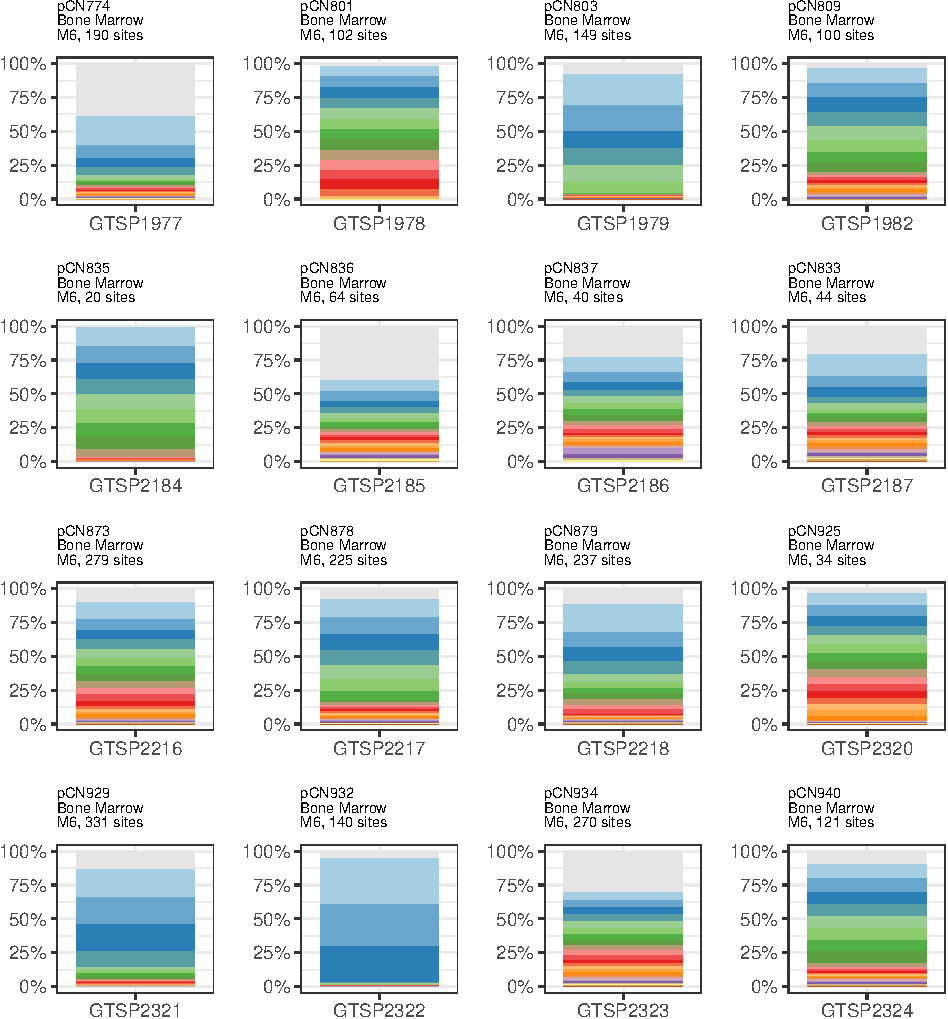
\includegraphics{project.group2_files/figure-latex/unnamed-chunk-3-1.pdf}

\newpage

\emph{Figure 2 (continued).}

\vspace{0.50cm}

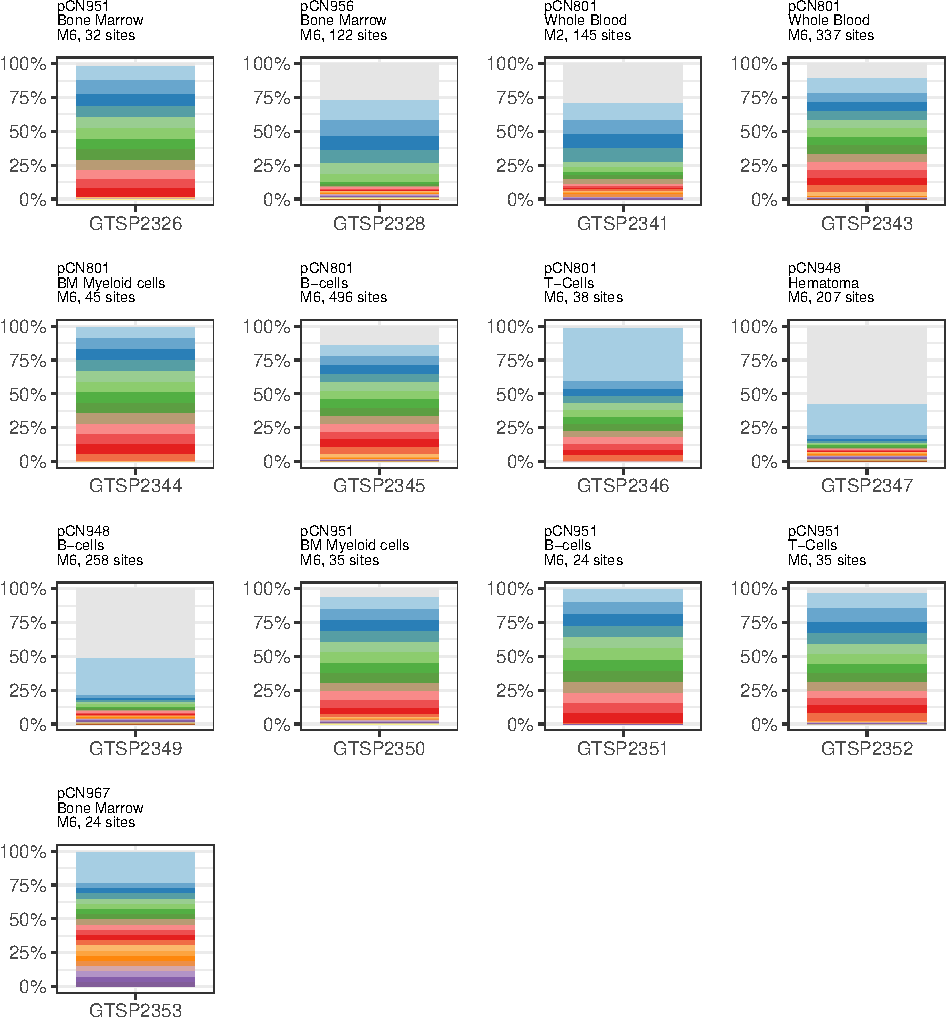
\includegraphics{project.group2_files/figure-latex/unnamed-chunk-4-1.pdf}

\newpage

\section{Expanded clones}\label{expanded-clones}

Table 2 below lists clones with relative clonal abundances \(\geq\)
20\%. The estimated number of cells harboring each integration
(Abundance) is shown for context.

\vspace{1.0cm}

\emph{Table 2.}

\begin{table}[H]
\centering\rowcolors{2}{gray!6}{white}

\resizebox{\linewidth}{!}{
\begin{tabular}{llllllrl}
\hiderowcolors
\toprule
Subject & Organism & Time point & Cell type & Position & Relative abundance & Abundance & Nearest gene\\
\midrule
\showrowcolors
pCN774 & mouse & M6 & Bone Marrow & chr1-21011655 & 21.02\% & 99 & Tram2\\
pCN803 & mouse & M6 & Bone Marrow & chr3+60155698 & 22.64\% & 461 & Mbnl1\\
pCN879 & mouse & M6 & Bone Marrow & chr15+44227316 & 20.85\% & 829 & Nudcd1\\
pCN929 & mouse & M6 & Bone Marrow & chr9+100734703 & 20.67\% & 669 & Stag1\\
pCN929 & mouse & M6 & Bone Marrow & chrX-126866229 & 20.02\% & 648 & Diaph2\\
pCN932 & mouse & M6 & Bone Marrow & chr12+80277915 & 33.13\% & 807 & Rdh11\\
pCN932 & mouse & M6 & Bone Marrow & chr8-66234933 & 31.53\% & 768 & Sgo2b\\
pCN932 & mouse & M6 & Bone Marrow & chr8+9405148 & 26.56\% & 647 & Fam155a\\
pCN801 & mouse & M6 & T-Cells & chr5-90109547 & 39.80\% & 780 & Adamts3\\
pCN948 & mouse & M6 & Hematoma & chr1-21011655 & 22.75\% & 76 & Tram2\\
pCN948 & mouse & M6 & B-cells & chr1-21011655 & 27.19\% & 143 & Tram2\\
\bottomrule
\end{tabular}}
\rowcolors{2}{white}{white}
\end{table}

\newpage

\section{Mapping of integration site
positions}\label{mapping-of-integration-site-positions}

Integration events were observerd across all mouse subject chromosomes
(Figure 3).

\vspace{1.0cm}

\emph{Figure 3}

\vspace{0.25cm}

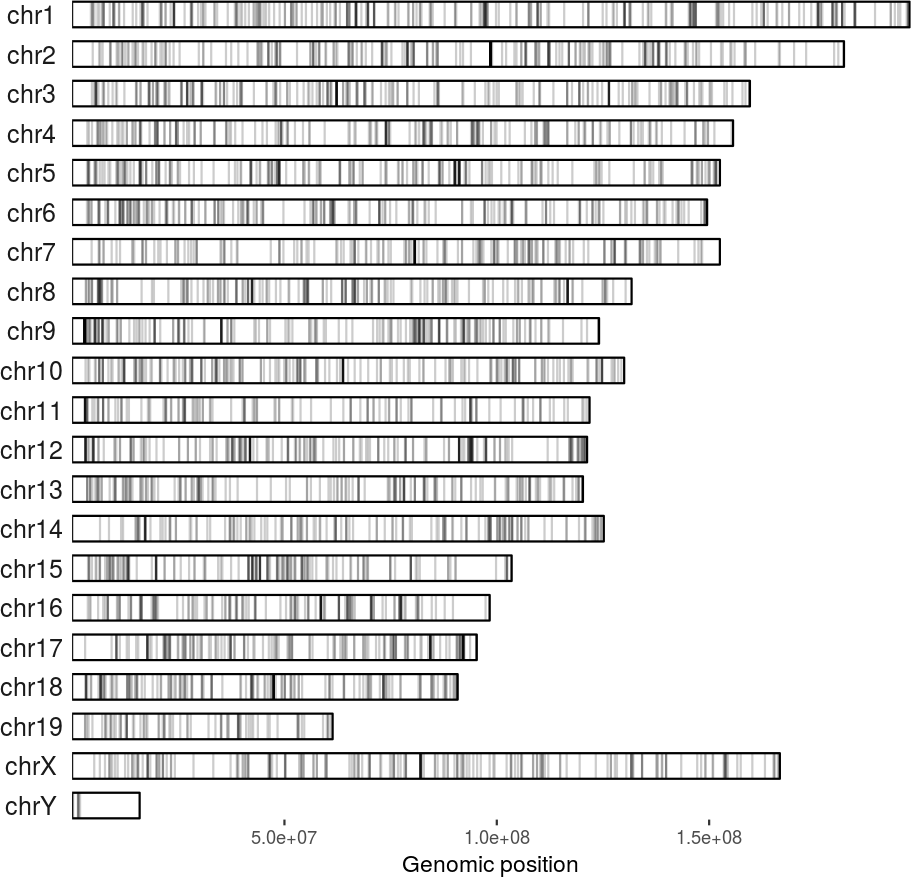
\includegraphics{project.group2_files/figure-latex/fig3a-1.png}

\newpage

\section{Mouse transplant trials}\label{mouse-transplant-trials}

The positions of identified integration sites from cell transplant
trials with nine pairs of mice are shown in Figure 4a (donor mice) and
Figure 4b (recipient mice). The gRxCluster software package did not
identify clusters of integration sites between donor and recipient mice
with a false discovery rate of \(\leq\) 10\%. The relative clonal
abundances of samples from the transplant trials are shown in Figure 5
where donor mice are shown on the left and recipient mice are shown on
the right. Integration sites are denoted by both nearest gene and
genomic coordinate and annotated with an asterisk (*) if located within
transcription units and with a tilda (\textasciitilde{}) if the
integration site is within 50 KB of an oncogene. Below each abundance
plot is a Fisher's exact test for the enrichment of oncogenes. None of
the tests returned a significant result. Instances where no integration
sites were identified in the recipient mouse are listed as `NA'. The
clonal abundances of clones found in both donor and recipient mice is
shown in Table S2. The identification of relatively few persistent
clones is likely due to sequencing experiments sampling only a subset of
existing integration sites and a number of samples with low vector copy
numbers (Figures 4B \& S3).

\vspace{0.5cm}

\emph{Figure 4}

\vspace{0.25cm}

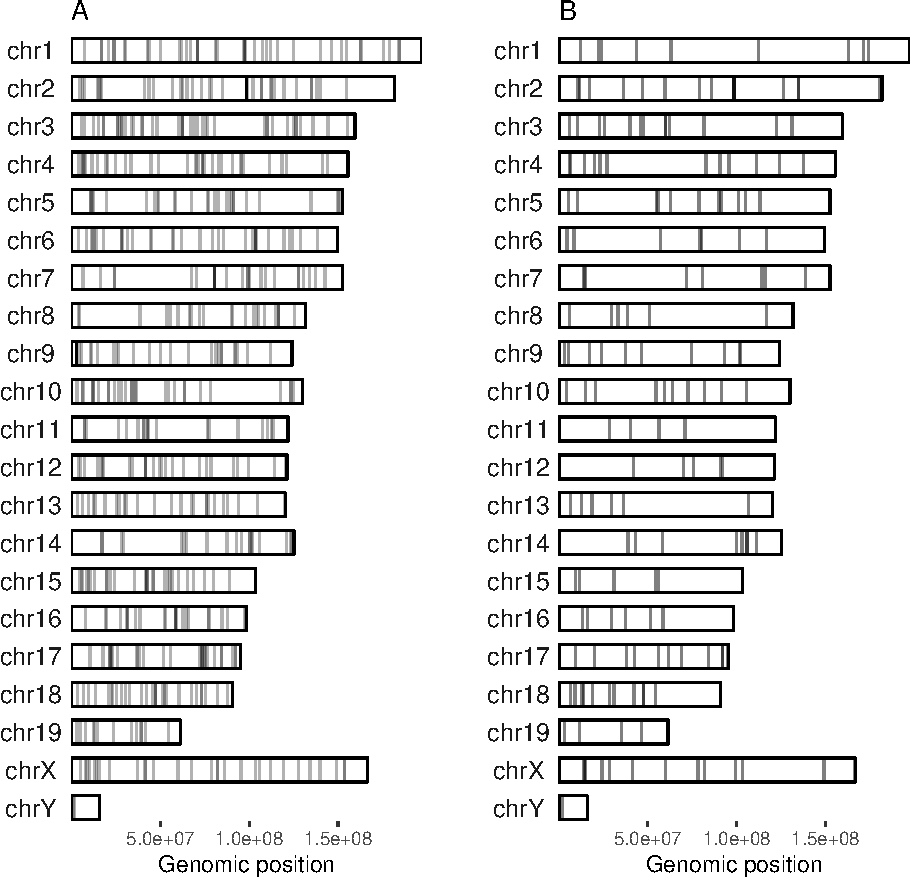
\includegraphics{project.group2_files/figure-latex/transplantSites-1.pdf}

\newpage

Figure 5a.

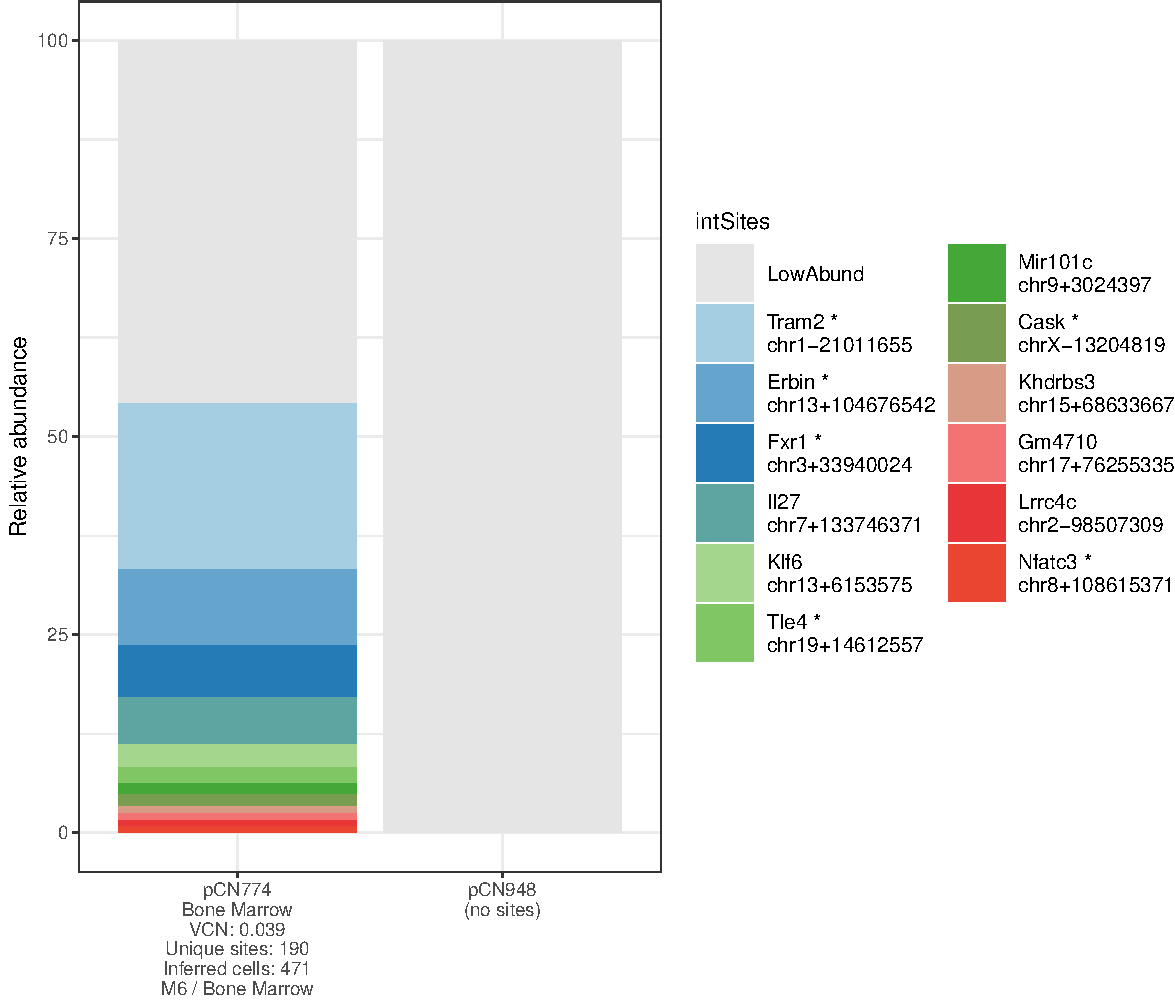
\includegraphics{project.group2_files/figure-latex/unnamed-chunk-5-1.pdf}
\vspace{1.0cm}

\begin{table}[!h]

\caption{\label{tab:unnamed-chunk-5}Fisher's exact p-value: 1.000}
\centering
\begin{tabular}[t]{lrr}
\toprule
  & Not near onco & Near onco\\
\midrule
pCN774 & 187 & 3\\
NA & 0 & 0\\
\bottomrule
\end{tabular}
\end{table}

\newpage

Figure 5b.

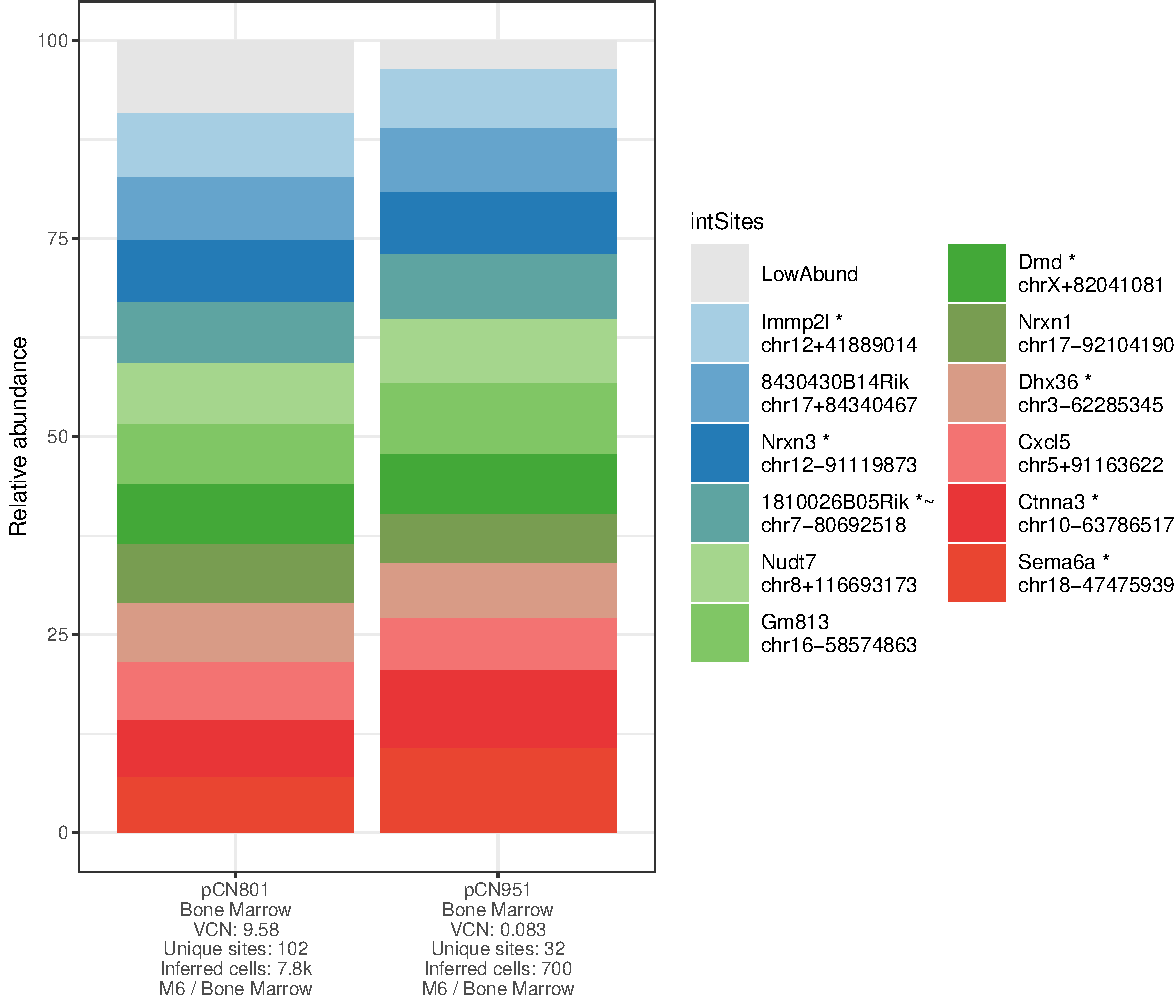
\includegraphics{project.group2_files/figure-latex/unnamed-chunk-5-2.pdf}
\vspace{1.0cm}

\begin{table}[!h]

\caption{\label{tab:unnamed-chunk-5}Fisher's exact p-value: 1.000}
\centering
\begin{tabular}[t]{lrr}
\toprule
  & Not near onco & Near onco\\
\midrule
pCN801 & 96 & 6\\
pCN951 & 31 & 1\\
\bottomrule
\end{tabular}
\end{table}

\vspace{2.0cm} \fontsize{10}{10}\selectfont
\(\bullet\) Integration at chr7-80692518, near 1810026B05Rik, is 6 KB
upstream of oncogene Chd2. \fontsize{12}{16}\selectfont

\newpage

Figure 5c.

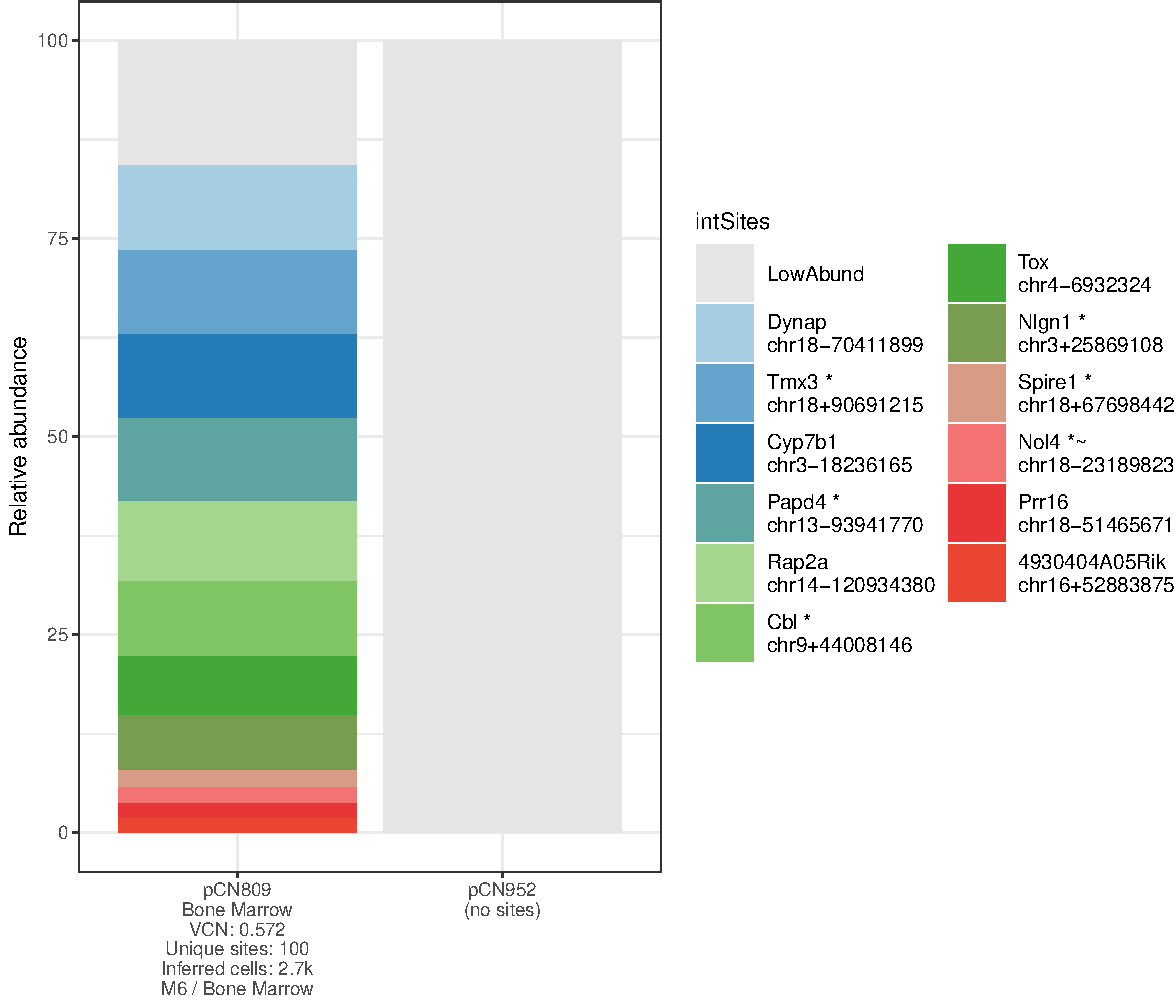
\includegraphics{project.group2_files/figure-latex/unnamed-chunk-5-3.pdf}
\vspace{1.0cm}

\begin{table}[!h]

\caption{\label{tab:unnamed-chunk-5}Fisher's exact p-value: 1.000}
\centering
\begin{tabular}[t]{lrr}
\toprule
  & Not near onco & Near onco\\
\midrule
pCN809 & 94 & 6\\
NA & 0 & 0\\
\bottomrule
\end{tabular}
\end{table}

\newpage

Figure 5d.

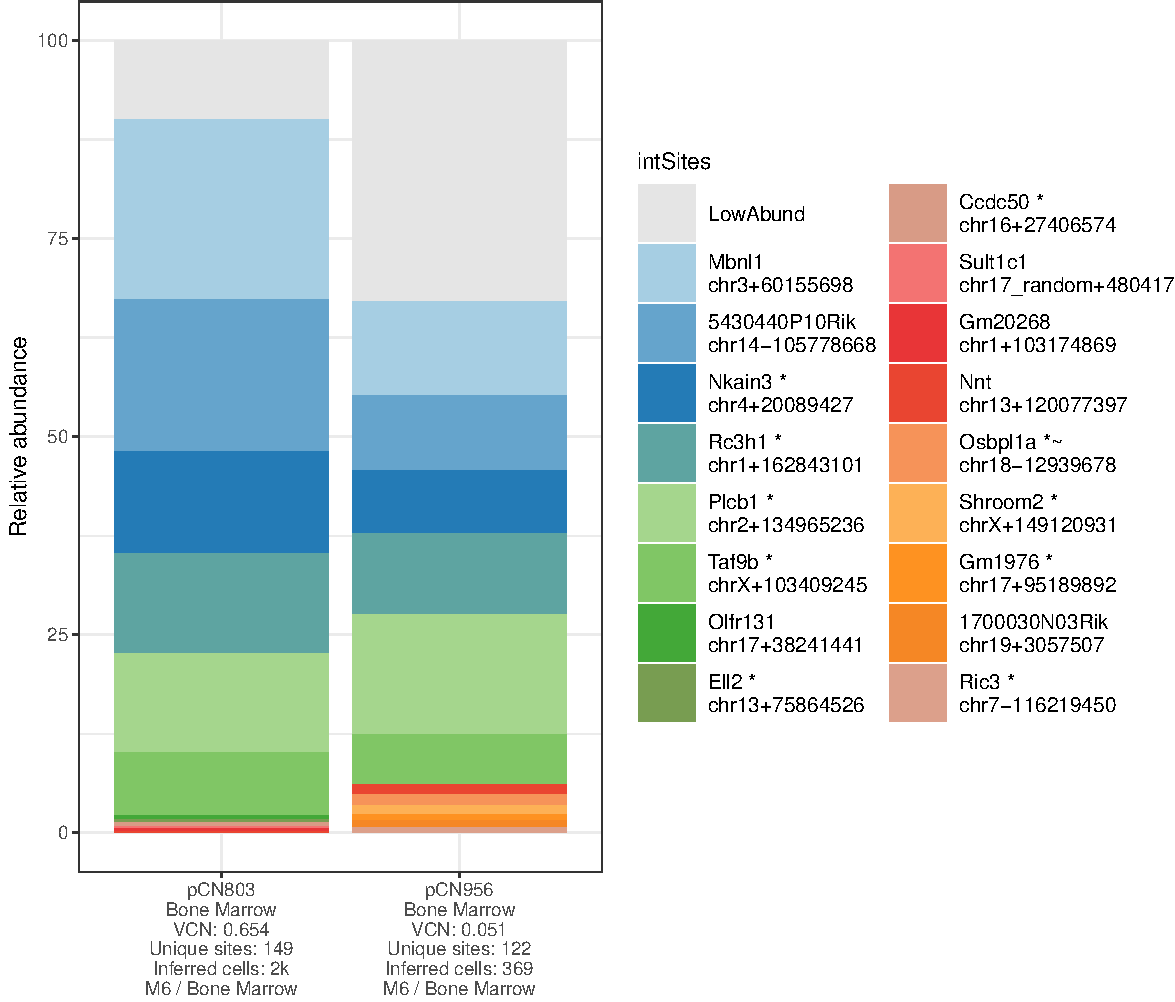
\includegraphics{project.group2_files/figure-latex/unnamed-chunk-5-4.pdf}
\vspace{1.0cm}

\begin{table}[!h]

\caption{\label{tab:unnamed-chunk-5}Fisher's exact p-value: 0.355}
\centering
\begin{tabular}[t]{lrr}
\toprule
  & Not near onco & Near onco\\
\midrule
pCN803 & 141 & 8\\
pCN956 & 119 & 3\\
\bottomrule
\end{tabular}
\end{table}

\newpage

Figure 5e.

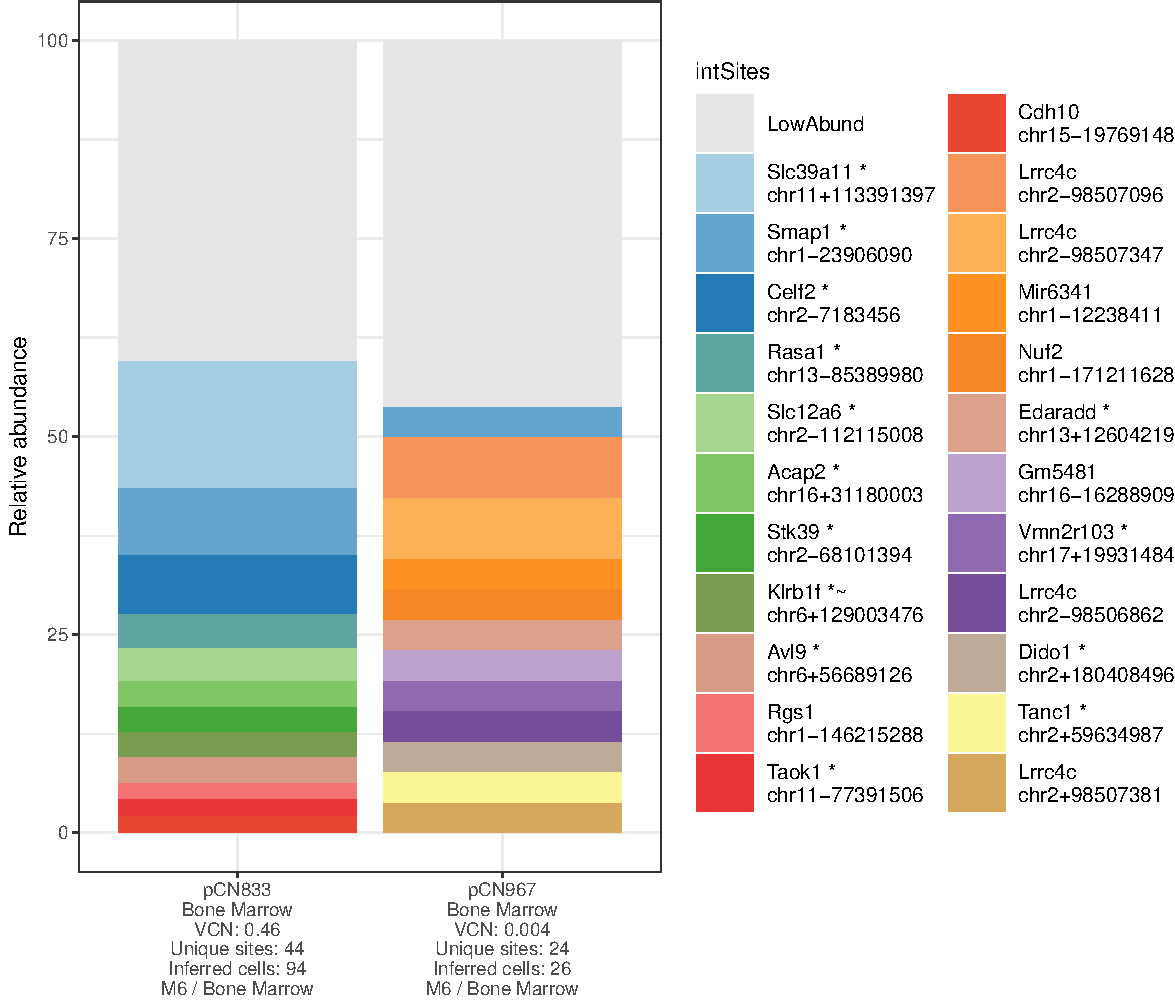
\includegraphics{project.group2_files/figure-latex/unnamed-chunk-5-5.pdf}
\vspace{1.0cm}

\begin{table}[!h]

\caption{\label{tab:unnamed-chunk-5}Fisher's exact p-value: 0.547}
\centering
\begin{tabular}[t]{lrr}
\toprule
  & Not near onco & Near onco\\
\midrule
pCN833 & 41 & 3\\
pCN967 & 24 & 0\\
\bottomrule
\end{tabular}
\end{table}

\newpage

\newpage

\textbf{Analyst}


\includegraphics[width=4.04in]{./data/Everett_signature}

John K. Everett, Ph.D.

\vspace{0.5cm}

\textbf{Laboratory director}

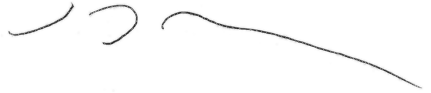
\includegraphics[width=5.99in]{./data/Bushman_signature}

Frederic D. Bushman, Ph.D.

\vspace{2.0cm}

\section{References}\label{references}

\begin{enumerate}
\def\labelenumi{\arabic{enumi}.}
\tightlist
\item
  RTCGD: retroviral tagged cancer gene database. Akagi K, Suzuki T,
  Stephens RM, Jenkins NA, Copeland NG. Nucleic Acids Res. 2004 Jan
  1;32(Database issue):D523-7.
\end{enumerate}

\vspace{0.1cm}

\begin{enumerate}
\def\labelenumi{\arabic{enumi}.}
\setcounter{enumi}{1}
\tightlist
\item
  Distribution of Lentiviral Vector Integration Sites in Mice Following
  Therapeutic Gene Transfer to Treat \(\beta\)-thalassemia. Ronen K,
  Negre O, Roth S, Colomb C, Malani N, Denaro M, Brady T, Fusil F,
  Gillet-Legrand B, Hehir K, Beuzard Y, Leboulch P, Down JD, Payen E,
  Bushman FD. Mol Ther. 2011 Jul;19(7):1273-86.
\end{enumerate}

\vspace{0.1cm}

\begin{enumerate}
\def\labelenumi{\arabic{enumi}.}
\setcounter{enumi}{2}
\tightlist
\item
  Estimating abundances of retroviral insertion sites from DNA fragment
  length data. Berry CC, Gillet NA, Melamed A, Gormley N, Bangham CR,
  Bushman FD. Bioinformatics. 2012 Mar 15;28(6):755-62.
\end{enumerate}

\vspace{0.1cm}

\begin{enumerate}
\def\labelenumi{\arabic{enumi}.}
\setcounter{enumi}{3}
\tightlist
\item
  INSPIIRED: A Pipeline for Quantitative Analysis of Sites of New DNA
  Integration in Cellular Genomes. Sherman E, Nobles C, Berry CC, Six E,
  Wu Y, Dryga A, Malani N, Male F, Reddy S, Bailey A, Bittinger K,
  Everett JK, Caccavelli L, Drake MJ, Bates P, Hacein-Bey-Abina S,
  Cavazzana M, Bushman FD. Mol Ther Methods Clin Dev. 2016 Dec
  18;4:39-49.
\end{enumerate}

\newpage

\section{Supplementary tables and
figures}\label{supplementary-tables-and-figures}

\subsection{Numbers of inferred cells and integration sites identified
in provided
samples}\label{numbers-of-inferred-cells-and-integration-sites-identified-in-provided-samples}

\emph{Table S1.}\\

\begin{table}[H]
\centering\rowcolors{2}{gray!6}{white}

\resizebox{\linewidth}{!}{
\begin{tabular}{llllrlll}
\hiderowcolors
\toprule
Organism & GTSP & Subject & Cell type & VCN & Time point & Number inferred cells & Number of intSites\\
\midrule
\showrowcolors
mouse & GTSP1977 & pCN774 & Bone Marrow & 0.039 & M6 & 471 & 190\\
mouse & GTSP1978 & pCN801 & Bone Marrow & 9.580 & M6 & 7,842 & 102\\
mouse & GTSP1979 & pCN803 & Bone Marrow & 0.654 & M6 & 2,036 & 149\\
mouse & GTSP1982 & pCN809 & Bone Marrow & 0.572 & M6 & 2,675 & 100\\
mouse & GTSP2184 & pCN835 & Bone Marrow & 1.481 & M6 & 393 & 20\\
mouse & GTSP2185 & pCN836 & Bone Marrow & 0.256 & M6 & 99 & 64\\
mouse & GTSP2186 & pCN837 & Bone Marrow & 0.138 & M6 & 66 & 40\\
mouse & GTSP2187 & pCN833 & Bone Marrow & 0.460 & M6 & 94 & 44\\
mouse & GTSP2216 & pCN873 & Bone Marrow & 0.786 & M6 & 4,681 & 279\\
mouse & GTSP2217 & pCN878 & Bone Marrow & 1.260 & M6 & 4,125 & 225\\
mouse & GTSP2218 & pCN879 & Bone Marrow & 1.061 & M6 & 3,976 & 237\\
mouse & GTSP2320 & pCN925 & Bone Marrow & 0.038 & M6 & 363 & 34\\
mouse & GTSP2321 & pCN929 & Bone Marrow & 2.000 & M6 & 3,237 & 331\\
mouse & GTSP2322 & pCN932 & Bone Marrow & 1.750 & M6 & 2,436 & 140\\
mouse & GTSP2323 & pCN934 & Bone Marrow & 0.506 & M6 & 2,720 & 270\\
mouse & GTSP2324 & pCN940 & Bone Marrow & 0.137 & M6 & 1,431 & 121\\
mouse & GTSP2326 & pCN951 & Bone Marrow & 0.083 & M6 & 700 & 32\\
mouse & GTSP2328 & pCN956 & Bone Marrow & 0.051 & M6 & 369 & 122\\
mouse & GTSP2341 & pCN801 & Whole Blood & 1.300 & M2 & 533 & 145\\
mouse & GTSP2343 & pCN801 & Whole Blood & 3.020 & M6 & 4,356 & 337\\
mouse & GTSP2344 & pCN801 & BM Myeloid cells & 7.950 & M6 & 8,411 & 45\\
mouse & GTSP2345 & pCN801 & B-cells & 2.690 & M6 & 7,174 & 496\\
mouse & GTSP2346 & pCN801 & T-Cells & 1.100 & M6 & 1,960 & 38\\
mouse & GTSP2347 & pCN948 & Hematoma & 0.018 & M6 & 334 & 207\\
mouse & GTSP2349 & pCN948 & B-cells & 0.019 & M6 & 526 & 258\\
mouse & GTSP2350 & pCN951 & BM Myeloid cells & 0.021 & M6 & 184 & 35\\
mouse & GTSP2351 & pCN951 & B-cells & 1.269 & M6 & 2,869 & 24\\
mouse & GTSP2352 & pCN951 & T-Cells & 0.026 & M6 & 326 & 35\\
mouse & GTSP2353 & pCN967 & Bone Marrow & 0.004 & M6 & 26 & 24\\
\bottomrule
\end{tabular}}
\rowcolors{2}{white}{white}
\end{table}

\newpage

\subsection{Persistence of clones in mouse BM transplant
trials}\label{persistence-of-clones-in-mouse-bm-transplant-trials}

\emph{Table S2.}

\begin{table}[H]
\centering\rowcolors{2}{gray!6}{white}

\begin{tabular}{lllll}
\hiderowcolors
\toprule
Donor & Recipient & Position & Donor cells & Recipient cells\\
\midrule
\showrowcolors
pCN801 & pCN951 & chr10-63786517 & 568 & 69\\
pCN801 & pCN951 & chr12-91119873 & 615 & 55\\
pCN801 & pCN951 & chr12+41889014 & 629 & 52\\
pCN801 & pCN951 & chr16-58574863 & 596 & 63\\
pCN801 & pCN951 & chr17-92104190 & 589 & 43\\
pCN801 & pCN951 & chr17+84340467 & 626 & 56\\
pCN801 & pCN951 & chr18-47475939 & 552 & 75\\
pCN801 & pCN951 & chr18-6677426 & 5 & 4\\
pCN801 & pCN951 & chr3-62285345 & 585 & 49\\
pCN801 & pCN951 & chr5-90109547 & 195 & 2\\
pCN801 & pCN951 & chr5+91163622 & 569 & 46\\
pCN801 & pCN951 & chr7-80692518 & 604 & 58\\
pCN801 & pCN951 & chr8+116693173 & 599 & 56\\
pCN801 & pCN951 & chrX+82041081 & 596 & 53\\
pCN803 & pCN956 & chr1+162843101 & 258 & 38\\
pCN803 & pCN956 & chr1+43686997 & 1 & 1\\
pCN803 & pCN956 & chr10-20694821 & 2 & 1\\
pCN803 & pCN956 & chr10+54685831 & 1 & 1\\
pCN803 & pCN956 & chr10+72683496 & 1 & 2\\
pCN803 & pCN956 & chr12+75878946 & 4 & 1\\
pCN803 & pCN956 & chr13+120077397 & 6 & 5\\
pCN803 & pCN956 & chr14-105778668 & 392 & 35\\
pCN803 & pCN956 & chr17+38241441 & 10 & 2\\
pCN803 & pCN956 & chr17+55932173 & 1 & 1\\
pCN803 & pCN956 & chr17+95189892 & 2 & 3\\
pCN803 & pCN956 & chr18-42192342 & 1 & 1\\
pCN803 & pCN956 & chr19+3057507 & 2 & 3\\
pCN803 & pCN956 & chr2+126512656 & 6 & 2\\
pCN803 & pCN956 & chr2+134965236 & 254 & 56\\
pCN803 & pCN956 & chr3-25751852 & 1 & 1\\
\bottomrule
\end{tabular}
\rowcolors{2}{white}{white}
\end{table}

\newpage

\subsection{Sequencing depth}\label{sequencing-depth}

Identified integration site are shown as colored squares that are
positioned by the number of reads leading to their identification.

\emph{Figure S3.}

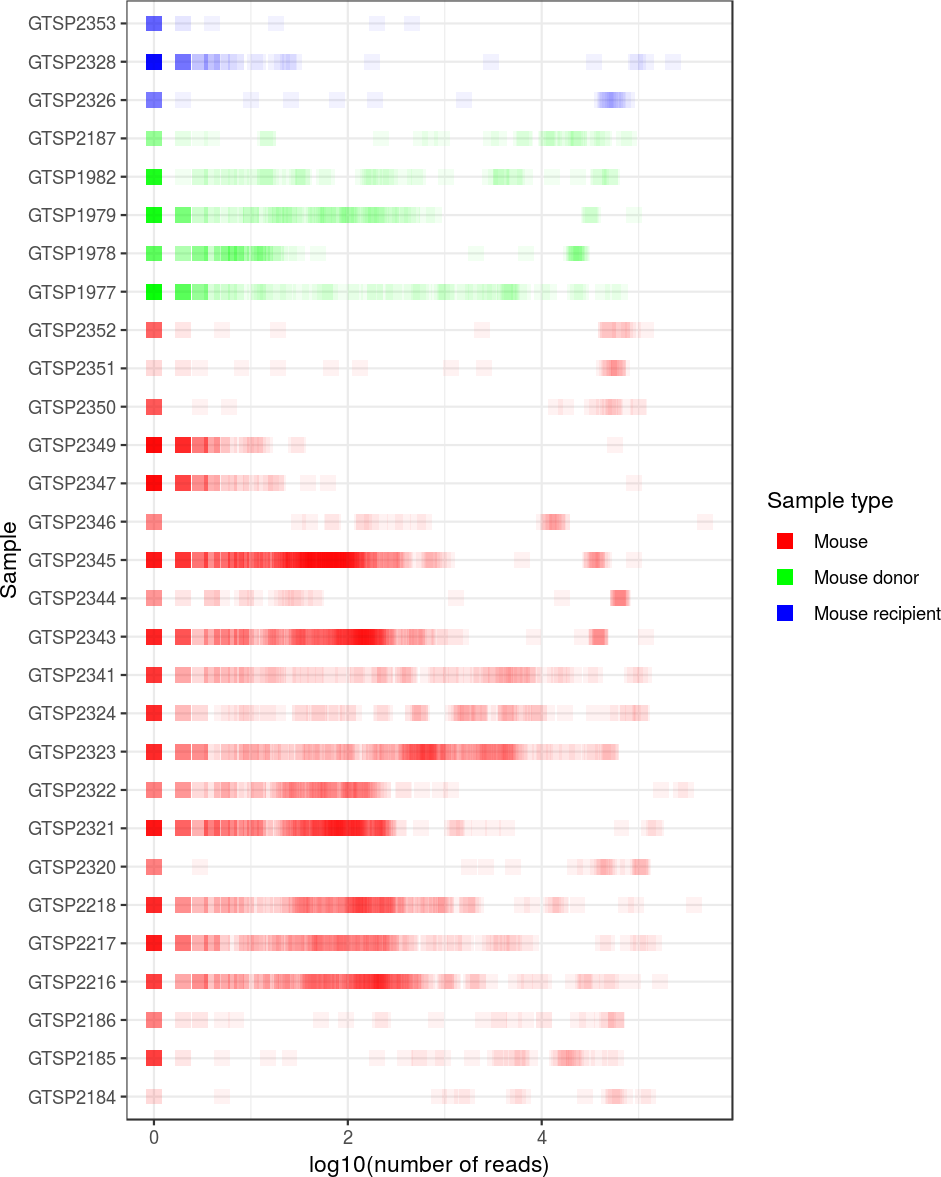
\includegraphics{project.group2_files/figure-latex/FigS3cont-1.png}


\end{document}
